% Options for packages loaded elsewhere
\PassOptionsToPackage{unicode}{hyperref}
\PassOptionsToPackage{hyphens}{url}
%
\documentclass[
]{article}
\usepackage{amsmath,amssymb}
\usepackage{iftex}
\ifPDFTeX
  \usepackage[T1]{fontenc}
  \usepackage[utf8]{inputenc}
  \usepackage{textcomp} % provide euro and other symbols
\else % if luatex or xetex
  \usepackage{unicode-math} % this also loads fontspec
  \defaultfontfeatures{Scale=MatchLowercase}
  \defaultfontfeatures[\rmfamily]{Ligatures=TeX,Scale=1}
\fi
\usepackage{lmodern}
\ifPDFTeX\else
  % xetex/luatex font selection
\fi
% Use upquote if available, for straight quotes in verbatim environments
\IfFileExists{upquote.sty}{\usepackage{upquote}}{}
\IfFileExists{microtype.sty}{% use microtype if available
  \usepackage[]{microtype}
  \UseMicrotypeSet[protrusion]{basicmath} % disable protrusion for tt fonts
}{}
\makeatletter
\@ifundefined{KOMAClassName}{% if non-KOMA class
  \IfFileExists{parskip.sty}{%
    \usepackage{parskip}
  }{% else
    \setlength{\parindent}{0pt}
    \setlength{\parskip}{6pt plus 2pt minus 1pt}}
}{% if KOMA class
  \KOMAoptions{parskip=half}}
\makeatother
\usepackage{xcolor}
\usepackage[margin=1in]{geometry}
\usepackage{graphicx}
\makeatletter
\def\maxwidth{\ifdim\Gin@nat@width>\linewidth\linewidth\else\Gin@nat@width\fi}
\def\maxheight{\ifdim\Gin@nat@height>\textheight\textheight\else\Gin@nat@height\fi}
\makeatother
% Scale images if necessary, so that they will not overflow the page
% margins by default, and it is still possible to overwrite the defaults
% using explicit options in \includegraphics[width, height, ...]{}
\setkeys{Gin}{width=\maxwidth,height=\maxheight,keepaspectratio}
% Set default figure placement to htbp
\makeatletter
\def\fps@figure{htbp}
\makeatother
\setlength{\emergencystretch}{3em} % prevent overfull lines
\providecommand{\tightlist}{%
  \setlength{\itemsep}{0pt}\setlength{\parskip}{0pt}}
\setcounter{secnumdepth}{-\maxdimen} % remove section numbering
\ifLuaTeX
  \usepackage{selnolig}  % disable illegal ligatures
\fi
\usepackage{bookmark}
\IfFileExists{xurl.sty}{\usepackage{xurl}}{} % add URL line breaks if available
\urlstyle{same}
\hypersetup{
  pdftitle={Encuentro 5: Documentación en RMarkdown},
  pdfauthor={Francisco Favieri \textbar{} Beatriz Soria},
  hidelinks,
  pdfcreator={LaTeX via pandoc}}

\title{Encuentro 5: Documentación en RMarkdown}
\usepackage{etoolbox}
\makeatletter
\providecommand{\subtitle}[1]{% add subtitle to \maketitle
  \apptocmd{\@title}{\par {\large #1 \par}}{}{}
}
\makeatother
\subtitle{Escuela de Verano: Taller de Introducción al procesamiento y
análisis de datos sobre mercado de trabajo con R}
\author{Francisco Favieri \textbar{} Beatriz Soria}
\date{}

\begin{document}
\maketitle

{
\setcounter{tocdepth}{2}
\tableofcontents
}
Material adaptado del trabajo realizado por Pablo Tiscornia

\subsubsection{R Markdown:
Introducción}\label{r-markdown-introducciuxf3n}

Los archivos R Markdown nos permiten combinar código, resultados y
texto. El objetivo de este encuentro es aprender a trabajar bajo dicho
entorno para facilitar tres aplicaciones:

\begin{itemize}
\tightlist
\item
  Documentar el trabajo que realizamos, incluyendo comentarios sobre los
  procedimientos.
\item
  Compartir código y resultados con personas que también trabajan en R.
\item
  Compartir resultados con personas que NO trabaja en R .
\end{itemize}

Las presentes notas de clase están basadas en el libro
\href{https://es.r4ds.hadley.nz/r-markdown.html}{R4DS} y las
\href{https://www.rstudio.com/resources/cheatsheets/}{cheatsheets}.
También se recomienda el libro
\href{https://bookdown.org/yihui/rmarkdown/}{R Markdown: The Definitive
Guide}.

\begin{center}\rule{0.5\linewidth}{0.5pt}\end{center}

\subsubsection{Requisitos}\label{requisitos}

Necesitamos instalar y cargar el paquete \textbf{rmarkdown}. Por lo
general, no hace falta hacerlo porque RStudio realiza esto
automáticamente.

\subsubsection{Markdown básico}\label{markdown-buxe1sico}

Se trata de un archivo de extensión \textbf{.Rmd}. Contiene en su
estructura tres tipos importantes de contenido:

\begin{itemize}
\tightlist
\item
  Un encabezado YAML (\emph{``Yet another markup lenguage''}) rodeado de
  - - -
\end{itemize}

\begin{verbatim}
---
title: "El título de nuestro informe"
date: Febrero 2025
output: html_document
---
\end{verbatim}

\begin{itemize}
\tightlist
\item
  Bloques de código de R rodeado de ```.
\end{itemize}

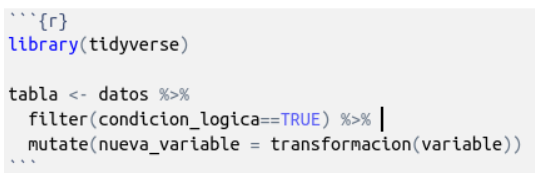
\includegraphics{img/Selection_008.png}

\begin{itemize}
\tightlist
\item
  Texto con formato
\end{itemize}

Cuando abrimos un archivo \textbf{.Rmd}, obtenemos una interfaz de
notebook donde el código y el output se encuentran intercalados (en
lugar de aparecer el output sólo en la consola, panel de plots y/o
modificaciones en el entorno de trabajo).

Los bloques de código se pueden ejecutar haciendo click en el ícono
\textbf{ejecutar} (el botón de \emph{Play} en la parte superior/derecha
del bloque), o presionando \texttt{Cmd/Ctrl\ +\ Shift\ +\ Enter}.
RStudio ejecuta el código y muestra los resultados incustrados en el
código.

Para producir un reporte completo que contenga todo el texto, código y
resultados, podemos clickear en \textbf{Knit} o presionar
\texttt{Cmd/Ctrl\ +\ Shift\ +\ K}. Esto mostrará el reporte en el panel
\emph{Viewer} y creará un archivo HTML independiente que podremos
compartir con otros.

\subsubsection{¿Qué es ``knitear''?}\label{quuxe9-es-knitear}

En el contexto de RMarkdown, es el proceso que convierte un archivo .Rmd
(R Markdown) en un documento final en formatos como HTML, PDF o Word.

Este proceso es gestionado por el paquete knitr y ejecuta el código R
dentro del documento, integrando los resultados en el texto final.

🔹 Para compilar manualmente un archivo .Rmd en RStudio, hacer clic en
el botón ``Knit'' o usar el comando. \textbf{``Knit''} significa
\textbf{``tejer''} el documento combinando texto, código y resultados en
un formato legible.

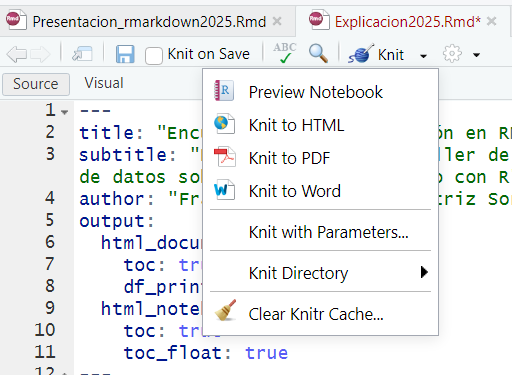
\includegraphics{img/knit.png}

\subsubsection{Formateo de texto}\label{formateo-de-texto}

La prosa en los archivos .Rmd está escrita en Markdown, una colección
simple de convenciones para dar formato a archivos de texto plano.
Markdown está diseñado para ser fácil de leer y fácil de escribir,
siendo también muy fácil de aprender. Del \emph{Cheatsheet}:

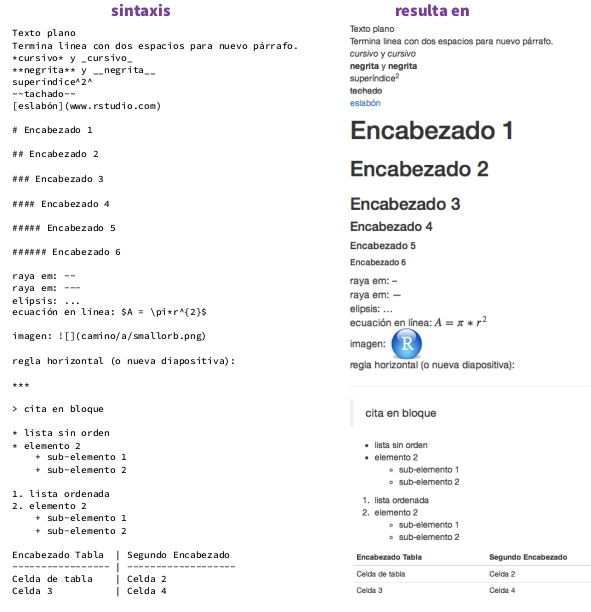
\includegraphics{img/Selection_001.png}

\begin{center}\rule{0.5\linewidth}{0.5pt}\end{center}

\subsubsection{Bloques de código}\label{bloques-de-cuxf3digo}

Como ya mencionamos, para ejecutar código dentro de un documento R
Markdown, necesitamos insertar un bloque (\emph{Chunk}). Hay tres
maneras para hacerlo:

\begin{itemize}
\tightlist
\item
  El atajo de teclado \texttt{Cmd/Ctrl\ +\ Alt\ +\ I}
\item
  El icono ``Insertar'' en la barra de edición
  (\texttt{Insert\ \textgreater{}\ R})
\item
  Tipear manualmente los delimitadores de bloque
  \texttt{\textasciigrave{}\textasciigrave{}\textasciigrave{}\{r\}} y
  \texttt{\textasciigrave{}\textasciigrave{}\textasciigrave{}}.
\end{itemize}

Obviamente, se recomienda usar el atajo de teclado porque, a largo
plazo, ahorra mucho tiempo. El código se puede seguir corriendo con
\texttt{Cmd/Ctrl\ +\ Enter} línea a línea. Sin embargo, los bloques de
código tienen otro atajo de teclado:
\texttt{Cmd/Ctrl\ +\ Shift\ +\ Enter}, que ejecuta todo el código en el
bloque.

Un bloque debería ser relativamente autónomo, y enfocado alrededor de
una sola tarea. Las siguientes secciones decriben el encabezado de
bloque que consiste en
\texttt{\textasciigrave{}\textasciigrave{}\textasciigrave{}\{r}, seguido
por un nombre opcional para el bloque, seguido entonces por
\textbf{opciones separadas por comas}, y concluyendo con \texttt{\}}.
Inmediatamente después sigue tu código de R el bloque y el fin del
bloque se indica con un
\texttt{\textasciigrave{}\textasciigrave{}\textasciigrave{}} final.

Hay un nombre de bloque que tiene comportamiento especial:
\texttt{setup}. Cuando nos encontramos en modo notebook, el bloque
llamado setup se ejecutará automáticamente una vez, antes de ejecutar
cualquier otro código.

\subsubsection{Opciones en los bloques de
código}\label{opciones-en-los-bloques-de-cuxf3digo}

La salida de los bloques puede personalizarse con \textbf{options},
argumentos suministrados en el encabezado del bloque. Knitr provee casi
60 opciones para que puedas usar para personalizar tus bloques de
código, la lista completa puede verse en
\url{http://yihui.name/knitr/options/}.

Las que más utilizamos nosotros son:

\begin{itemize}
\item
  \texttt{eval\ =\ FALSE} evita que código sea evaluado. (Y obviamente
  si el código no es ejecutado no se generaran resultados). Esto es útil
  para mostrar códigos de ejemplo, o para deshabilitar un gran bloque de
  código sin comentar cada línea.
\item
  \texttt{include\ =\ FALSE} ejecuta el código, pero no muestra el
  código o los resultados en el documento final. Usa esto para el código
  de configuracion que no quieres que abarrote tu reporte.
\item
  \texttt{echo\ =\ FALSE} evita que se vea el código, pero no los
  resultados en el archivo final. Utiliza esto cuando quieres escribir
  reportes enfocados a personas que no quieren ver el código subyacente
  de R.
\item
  \texttt{message\ =\ FALSE} o \texttt{warning\ =\ FALSE} evita que
  aparezcan mensajes o advertencias en el archivo final.
\item
  \texttt{results\ =\ \textquotesingle{}hide\textquotesingle{}} oculta
  el output impreso;
  \texttt{fig.show\ =\ \textquotesingle{}hide\textquotesingle{}} oculta
  gráficos.
\item
  \texttt{error\ =\ TRUE} causa que el render continúe incluso si el
  código devuelve un error. Esto es algo que raramente querés incluir en
  la version final de tu reporte.
\end{itemize}

Contamos con algunas de estas opciones en el menú de
\textbf{Configuración} en la parte superior-derecha del \emph{Chunk} de
código.

\subsubsection{Formatos}\label{formatos}

Hasta ahora vimos R Markdown para producir documentos HTML:

\begin{verbatim}
---
title: "Clase"  
output: html_document
---
\end{verbatim}

Para sobrescribir los parámetros predeterminados se necesita usar un
campo de output extendido. Por ejemplo, si queremos generar un
\texttt{html\_document} con una tabla de contenido flotante, usamos:

\begin{verbatim}
---
title: "Clase"
output:
  html_document:
    toc: true
    toc_float: true
---
\end{verbatim}

Para los \texttt{html\_document} otra opción es hacer que los fragmentos
de código estén escondidos por defecto, pero visibles con un
\emph{click}:

\begin{verbatim}
---
title: "Clase"
output:
  html_document:
    code_folding: hide
---
\end{verbatim}

\subsubsection{Otros formatos}\label{otros-formatos}

Hay todo un número de variaciones básicas para generar diferentes tipos
de documentos:

\begin{itemize}
\item
  \texttt{pdf\_document} crea un PDF con LaTeX (un sistema de código
  abierto de composición de textos), que necesitarás instalar. RStudio
  te notificará si no lo tienes.
\item
  \texttt{word\_document} para documentos de Microsoft Word (.docx).
\item
  \texttt{odt\_document} para documentos de texto OpenDocument (.odt).
\end{itemize}

y más!

\subsubsection{Notebooks}\label{notebooks}

Un notebook, \texttt{html\_notebook} (``cuaderno'' en español), es una
variación de un \texttt{html\_document}. Las salidas de los dos
documentos son muy similares, pero tienen propósitos distintos. Un
\texttt{html\_document} está enfocado en la comunicación con los
encargados de la toma de decisiones, mientras que un notebook está
enfocado en colaborar con otros científicos de datos. Estos propósitos
diferentes llevan a usar la salida HTML de diferentes maneras. Ambas
salidas HTML contendrán la salida renderizada, pero \textbf{el notebook
también contendrá el código fuente completo}. Esto significa que podemos
usar el archivo \texttt{.nb.html} generado por el notebook de dos
maneras:

\begin{itemize}
\item
  Podemos verlo en un navegador web, y ver la salida generada. A
  diferencia del \texttt{html\_document}, esta renderización siempre
  incluye una copia incrustada del código fuente que lo generó.
\item
  Podemos editarlo en RStudio. Cuando abramos un archivo
  \texttt{.nb.html}, RStudio automáticamente recreará el archivo
  \texttt{.Rmd} que lo creó.
\end{itemize}

\subsubsection{Publicar}\label{publicar}

Desde RStudio tenemos la posibilidad de publicar nuestros Markdown en
\href{https://rpubs.com/}{RPubs} de forma gratuita, desde el botón
\textbf{Publish document}. Todo lo que subamos a nuestra cuenta de RPubs
será público.

\begin{center}\rule{0.5\linewidth}{0.5pt}\end{center}

\section{Práctica}\label{pruxe1ctica}

\begin{enumerate}
\def\labelenumi{\arabic{enumi})}
\tightlist
\item
  Crear un informe que contenga:
\end{enumerate}

\begin{itemize}
\tightlist
\item
  \textbf{En TEXTO:}

  \begin{itemize}
  \tightlist
  \item
    Una estructura mínima de texto (Título, consigna, descripción de las
    tareas realizadas y muy breve conclusión)
  \end{itemize}
\item
  \textbf{En CÓDIGO:}

  \begin{itemize}
  \tightlist
  \item
    Carga de librerías (no mostrar el código en el reporte)
  \item
    Importación de datos (mostrar el código en el reporte)
  \item
    Algún procesamiento mínimo como filtrar, seleccionar, generar un
    tabulado, etc. (mostrar el código y el resultado en el reporte)
  \end{itemize}
\item
  \emph{Extra}: Incluir un gráfico
\end{itemize}

\end{document}
